\chapter{الجداول (\textenglish{Arrays})}

هذا الفصل هو ملحق مباشر للفصل المتعلق بالمؤشرات، و سيعلّمك أهميتها أكثر. إن كنت تعتقد بأنك قادر على تفادي المؤشرات فأنت مخطئ ! هي في كلّ مكان في لغة الـ\textenglish{C}. لقد حذّرتك !

سنتعلم في هذا الفصل كيف ننشئ متغيرات من نوع "جداول". الجدوال مهمّة للغاية في لغة الـ\textenglish{C} لأنها تساعد في تنظيم سلسلة من القيم.

نبدأ هذا الفصل ببعض الشروحات و التفسيرات حول كيفية عمل الجداول في الذاكرة (سأقدم لك الكثير من المخططات التفسيرية). هذه المقدمات حول الذاكرة مهمة جداً : ستساعدك في في معرفة عمل الجداول. فمن المستحسن أن يعرف المبرمج ما يقوم به كي يتحكم في برامجه أكثر، أليس كذلك ؟

\section{الجداول في الذاكرة}

\textit{"الجداول هي تتابع متغيرات من نفس النوع، موجودة في مكان متواصل من الذاكرة."}

أعرف أن هذا التعريف يشبه قليلا تعريف القاموس. لهذا فسأوضح بطريقة أخرى، فعلياّّ، الجدول عبارة عن "متغيّرات ضخمة" يمكن لها أن تحتوي على أعداد كبيرة من نفس النوع
(\InlineCode{char}،
\InlineCode{long}،
\InlineCode{int}،
\InlineCode{double}...).

للجدول طول محدد. يمكنه أن يكون 2، 3، 10 خانات، 150، 2500 خانة، أنت من يحدد العدد. المخطط التالي مثال عن جدول يحجز 4 خانات بدءاً بالعنوان 1600 :

\begin{figure}[H]
	\centering
	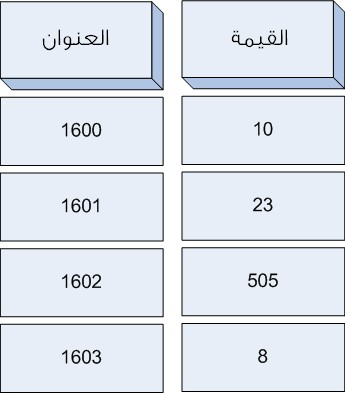
\includegraphics[width=0.4\textwidth]{Chapter_II-3_Array-Adresses}
\end{figure}

عندما تطلب إنشاء جدول يحجز 4 خانات في الذاكرة، سيطلب برنامجك من نظام التشغيل أن يسمح له باستغلال 4 خانات في الذاكرة، و يجب ان تكون هذه الخانات متتالية يعني الواحدة بجانب الأخرى. و كما ترى أعلاه فالخانات متتابعة 1600، 1601، 1602، 1603 فلا يوجد "فراغ" بينها.

أخيراً، كل خانة تحتوي عددا من نفس النوع. فإن كان الجدول من نوع
\InlineCode{int}
فإن كلّ خانة يجب أن تحتوي عددا من نوع
\InlineCode{int}.
و بهذا نفهم أنه لا يمكننا وضع نوع
\InlineCode{int}
مع
\InlineCode{double}
في الجدول نفسه.

و كتلخيص، هذا أهم ما يجب أن تعرفه بخصوص الجداول :

\begin{itemize}
  \item عندما يتم إنشاء جدول، يأخذ مكانا متواصلاً في الذاكرة. بحيث تكون الخانات متجاورة الواحدة تلو الأخرى.
  \item كل خانات الجدول تكون من نفس النوع، فجدول
الـ\InlineCode{int}
يمكن أن يحمل فقط
\InlineCode{int}،
و لا أي نوع آخر.
\end{itemize}

\section{تعريف جدول}

كي نبدأ سننشئ جدولا من 4 أعداد من نوع
\InlineCode{int} :

\begin{Csource}
int table[4];
\end{Csource}

هذا كلّ شيء. يكفي إذن أن تضيف قوسين مربعين
(\InlineCode{[}
و
\InlineCode{]})
عدد الخانات التي تريد أن يحجزها جدولك، و اعلم أنه لا يوجد حدود (إلا إن تجاوزت الحدّ الذي تسمح به ذاكرة جهازك طبعا).

و لكن الآن، كيف نصل لخانة ما في الجدول ؟
هذا سهل، تكفي كتابة
\InlineCode{table[cellNumber]}.

\begin{critical}
 احذر : كل جدول يجب أن يبدأ بالفهرس
(\textenglish{Index})
رقم 0 ! جدولنا متكوّن من 4
\InlineCode{int}
إذن فالفهارس المتوفرة هي : 0، 1، 2 و 3. لا وجود للفهرس 4 في جدول من 4 خانات ! هذا مصدر أخطاء متداولة، فلا تغفل عنه !

\end{critical}

إذا كنت أريد أن أضع في جدولي نفس القيم التي في المخطط فبجب إذا أن أكتُب :

\begin{Csource}
int table[4];
table[0] = 10;
table[1] = 23;
table[2] = 505;
table[3] = 8;
\end{Csource}

\begin{question}
  لازلت لا أرى العلاقة بين المؤشرات و الجداول ؟
\end{question}

في الواقع، لو تكتب فقط
\InlineCode{table}
فستحصل على مؤشر، و هو مؤشر على الخانة الأولى من الجدول، قم باختبار التالي :

\begin{Csource}
int table[4];
printf("%d", table);
\end{Csource}

النتيجة ستظهر لك العنوان الذي يتواجد به
\InlineCode{table} :

\begin{Console}
1600
\end{Console}

بينما إذا قمت بوضع فهرس الخانة بين قوسين مربعين، فستحصل على القيمة :

\begin{Csource}
int table[4];
printf("%d", table[0]);
\end{Csource}

\begin{Console}
10
\end{Console}

نفس الشيء بالنسبة للفهارس الأخرى. بما أن
\InlineCode{table}
هو مؤشر، يمكننا استعمال الرمز
\InlineCode{*}
للحصول على القيمة الأولى :

\begin{Csource}
int table[4];
printf("%d", *table);
\end{Csource}

\begin{Console}
10
\end{Console}

يمكن أيضا الحصول على قيمة الخانة الثانية بكتابة
\InlineCode{*(table + 1)}
(أي عنوان الجدول + 1). لذا فهذان السطران متماثلان :

\begin{Csource}
table[1] // Returns the value of the second cell (the first is 0)
*(table + 1) // Same thing : returns the value of the second cell.
\end{Csource}

لذا فعند كتابة
\InlineCode{table[0]}،
فأنت تطلب قيمة الخانة التي تتواجد بعنوان الجدول + 0
خانة، أي 1600.\\
و إذا كتبت
\InlineCode{table[1]}
فإنك تطلب القيمة المتواجدة في عنوان الجدول + 1
خانة، أي 1601.\\
و هكذا من أجل الباقي.

\subsection{الجداول ذات الحجم المتغيّر}

هناك عدة نسخ من لغة
\textenglish{C}.\\
نسخة حديثة منها تدعى
\textenglish{C99}
تسمح بإنشاء جداول ذات حجم متغيّر. يعني أن حجم الجداول يمكن أن يكون معرّفا بمتغير.

\begin{Csource}
int size = 5;
int table[size];
\end{Csource}

إلا أن هذه الكتابة ليست مفهومة بالنسبة لكل الـمترجمات
(\textenglish{Compilers})
فبعضها تتوقف في السطر الثاني. إن لغة
الـ\textenglish{C}
الّتي اعلمك إياها منذ البداية (تدعى
\textenglish{C89})
لا تسمح بهذا النوع من الكتابات. و لذا يمكننا القول أن فعل هذه الأشياء أمر ممنوع.

يجب أن نتفق على شيء و هو : لا تملك الحق في وضع متغير بين القوسين المربعين من أجل تعريف حجم الجدول. حتى و إن كان المتغير ثابتا ! يجب على طول الجدول أن يأخذ قيمة ثابتة، و لهذا عليك أن تحدده كعدد :
\begin{Csource}
int table[5];
\end{Csource}

\begin{question}
   إذن \dots هل من الممنوع إنشاء جدول يعتمد حجمه على قيمة متغير ؟
\end{question}

بلى إنه ممكن حتى مع
\textenglish{C89}.
لكن لفعل هذا سنعتمد على تقنية أخرى (أكيدة أكثر و تعمل مع كل المترجمات) تدعى بـ\textbf{الحجز الحيّ}
(\textenglish{Dynamic allocation}).
سندرسها في مرحلة متقدمة من هذا الكتاب.

\section{تصفح جدول}

لنفرض أنني أريد الآن أن أُظهر كل قيم خانات الجدول.\\
يمكنني أن أستدعي الدالة
\InlineCode{printf}
بالقدر الذي يحتويه الجدول من خانات. لكن سيكون الأمر ثقيلاً و مليئاً بالتكرار، و تخيل حجم الشفرة المصدرية لو أننا أردنا إظهار قيم الجدول واحدة بواحدة !

الأحسن هو أن نستعين بحلقة. لم لا حلقة
\InlineCode{for}
؟ فهي الأنسب لتصفح الجداول :

\begin{Csource}
int main(int argc, char *argv[])
{
	int table[4], i = 0;
	table[0] = 10;
	table[1] = 23;
	table[2] = 505;
	table[3] = 8;
	for (i = 0 ; i < 4 ; i++)
	{
    		printf("%d\n", table[i]);
	}
	return 0;
}
\end{Csource}

\begin{Console}
10
23
505
8
\end{Console}

إن حلقتنا تتصفح الجدول بمساعدة متغير يسمى
\InlineCode{i}
(اسم شائع لدى المبرمجين يخص المتغير الذي يستخدم لتصفح جدول !).

إن الشيء العَمَلِيَّ خاصة، هو أنه بإمكاننا وضع متغير داخل قوسين مربعين بالفعل. فالمتغير كان ممنوعا في مرحلة إنشاء الجدول (لتعريف حجمه). لكن و لحسن الحظ، فهو مسموح من أجل "تصفح" الجدول، أي إظهار قيمه !\\
هنا قد نعطي المتغير
\InlineCode{i}
بشكل متتالي القيم 0، 1، 2، 3. بهذا سنقوم إذن بإظهار قيمة
\InlineCode{table[0]}،
\InlineCode{table[1]}،
\InlineCode{table[2]}
و
\InlineCode{table[3]} !

\begin{critical}
  إنتبه لعدم محاولة إظهار قيمة
\InlineCode{table[4]} !
فجدول من 4 خانات يتضمن الفهارس 0، 1، 2، 3 فقط. فإن حاولت عرض
\InlineCode{table[4]}
فإمّا أن تحصل على قيمة عشوائية، أو أن يظهر لك خطأ جميل، نظام التشغيل يوقف برنامجك فهو يحاول الوصول لعنوان لا ينتمي إليه.
\end{critical}

\subsection{تهيئة جدول}

الآن و مادمنا قد عرفنا كيف نتصفح جدولا، يمكننا أن نضبط كل قيمه على 0 باستخدام حلقة !

إن القيام بتصفح جدول لضبط كلّ قيمه على الصفر أمر يمكن القيام به بمستواك هذا :

\begin{Csource}
int main(int argc, char *argv[])
{
	int table[4], i = 0;
	// Initialization of the table
	for (i = 0 ; i < 4 ; i++)
	{
    		table[i] = 0;
	}
	// Displaying the values of the table to check
	for (i = 0 ; i < 4 ; i++)
	{
    		printf("%d\n", table[i]);
	}
	return 0;
}
\end{Csource}

\begin{Console}
0
0
0
0
\end{Console}

\subsection{طريقة أخرى للتهيئة}

يجب أن تعرف أنه هناك طريقة أخرى لإعطاء قيم ابتدائية لجدول في لغة الـ\textenglish{C}.\\
و هذه الطريقة تعمل بكتابة
\InlineCode{table[4] = \{value1, value2, value3, value4\}}.
ببساطة، تضع القيم بين حاضنتين واحدة تلو الاخرى و تفصل بينها بفواصل.

\begin{Csource}
int main(int argc, char *argv[])
{
	int table[4] = {0, 0, 0, 0}, i = 0;
	for (i = 0 ; i < 4 ; i++)
	{
    	printf("%d\n", table[i]);
	}
	return 0;
}
\end{Csource}

\begin{Console}
0
0
0
0
\end{Console}

و هناك أحسن من هذه الطريقة : بإمكانك تعريف القيم الخاصة بالخانات الأولى من الجدول و كل التي لم تُشر إليها ستُضبط على 0.

أي أنني إن قمت بكتابة التالي :

\begin{Csource}
int table[4] = {10, 23}; // Inserted values : 10, 23, 0, 0
\end{Csource}

الخانة 0 تأخذ القيمة 10 و الخانة 1 تأخذ القيمة 23 و كل الخانات المتبقية تأخذ القيمة 0 (افتراضياً).

كيف نضبط كل الجدول على الصفر بمعرفة هذا ؟\\
يكفي أن تضبط القيمة الأولى على 0، و كل القيم الاخرى غير المشار إليها تأخذ القيمة 0.

\begin{Csource}
int table[4] = {0}; // All the columns of the table will be initialised to 0
\end{Csource}

هذه التقنية لها شيء مميز و هو أنها تعمل مع أي جدول مهما كان حجمه (في هذا المثال نجحت الطريقة مع 4 خانات و ستنجح لو كان الجدول بـ100 خانة أيضا).

\begin{critical}
احذر، قد تصادفك الكتابة التالية :
\InlineCode{int table[4] = \{1\};}
و التي تعني إدخال القيم التالية في الجدول :
1، 0، 0، 0.\\
خلافاً لما يعتقده الكثير، لن يتم تهيئة كل خانات الجدول على 1. بل الخانة الأولى هي الوحيدة التي تضبط على 1 أما الباقي فعلى 0. لا يمكننا إذن القيام بتهيئة كل الجدول على القيمة 1 تلقائيّا، إلّا باستعمال حلقة.
\end{critical}

\section{تمرير جدول لدالة}

في كثير من الأوقات ستحتاج لإظهار محتوى كلّ الجدول، فلما لا نقوم بكتابة دالة تقوم بهذا ؟ بهذا ستكتشف كيف نمرر جدولا إلى دالة (و هذا يساعدني).

يتطلب الأمر أن تبعث معلومتين للدالة. الجدول (أي عنوان الجدول) و أيضا حجمه خاصّة !\\
بالفعل، يجب أن تكون دالتنا قادرة على تهيئة جدول مهما كان حجمه. لكن في دالتنا، أنت لا تعرف حجم جدولك و لهذا يجب أن ترسل متغيرا يحمل الاسم
\InlineCode{tableSize}
مثلا.

و كا قلت لك مسبقا، يمكننا إعتبار
\InlineCode{table}
مؤشرا، و لهذا يمكننا أن نرسله للدالة مثلما نرسل مؤشرا عاديا.

\begin{Csource}
// Prototype of the display function
void display(int *table, int tableSize);

int main(int argc, char *argv[])
{
	int table[4] = {10, 15, 3};
 	// We display the content of the table
	display(table, 4);
	return 0;
}

void display(int *table, int tableSize)
{
	int i;
	for (i = 0 ; i < tableSize; i++)
	{
    		printf("%d\n", table[i]);
	}
}
\end{Csource}

\begin{Console}
10
15
3
0
\end{Console}

الدالة غير مختلفة عن التي درسناها في فصل المؤشرات، فهي تأخذ كمعامل مؤشراً نحو
\InlineCode{int}
(جدولنا) و أيضا حجمه (مهم جدا كي نعرف متى تتوقف الحلقة !).\\
كل محتوى الجدول تُظهره الدالة بواسطة الحلقة.

لاحظ أنّه توجد طريقة أخرى للإشارة إلى أن الدالة تستقبل جدولا. بدلا من أن نشير أن الدالة تستقبل
\InlineCode{int *table}،
أكتب التالي :

\begin{Csource}
void display(int table[], int tableSize)
\end{Csource}

هذا يعني تماما نفس الشيء، و لكن وجود القوسين المربعين يُعلمان المبرمج بأن الدالة تأخذ جدولا و ليس مؤشرا عاديا و هذا يزيل الغموض.

شخصيا أستعمل دائما القوسين المربعين في دوالي لكي أُظهر بأن الدالة تنتظر جدولا. أنصحك باستعمال نفس الطريقة. ليس مهما وضع حجم الجدول بين القوسين المربعين هذه المرة.

\subsection{بعض التمارين !}

لدي أفكار متعددة عن تمارين متعلقة بالجداول ستساعدك على التدريب ! و فكرة التمارين هي إنشاء دوال تعمل على الجداول.

و كتحدي، ستجد هنا نصوص  التمارين فقط، و لن أعطي الإجابة كي أجبرك على الاجتهاد في إيجاد الحلول، فإن لم تستطع فيمكنك زيارة 
\href{http://www.siteduzero.com/forum-81-126-langage-c.html}{المنتديات} 
لطرح أسئلتك.

\subsubsection{التمرين 1}

أنشئ دالة
\InlineCode{tableSum}
ترجع مجموع القيم الموجودة في الجدول (استعمل
\InlineCode{return}
لإرجاع النتيجة) و  للمساعدة، هذا هو نموذج  الدالة :

\begin{Csource}
int tableSum(int table[], int tableSize);
\end{Csource}

\subsubsection{التمرين 2}

أنشئ دالة
\InlineCode{tableAverage}
تحسب و تُرجع معدّل القيم الموجودة في الجدول. تفضل النموذج :

\begin{Csource}
double tableAverage(int table[], int tableSize);
\end{Csource}

الدالة ترجع
\InlineCode{double}
فالمعدّل عادة هو قيمة عشرية.

\subsubsection{التمرين 3}

أنشئ دالة
\InlineCode{tableCopy}
التي تأخذ كمعاملات جدولين، حيث تقوم بنسخ محتوى الجدول الأول في الجدول الثاني، تفضل النموذج :

\begin{Csource}
void tableCopy(int originalTable[], int copyTable[], int tableSize);
\end{Csource}

\subsubsection{التمرين 4}

أنشئ دالّة
\InlineCode{tableMaximum}
دورها إسناد 0 لكلّ خانة جدول تحوي قيمة أكبر من القيمة العظمى. هذه الدالة تأخذ كمعاملات الجدول و العدد الأقصى المسموح به
(\InlineCode{maxValue}).
كلّ الخانات الّتي تملك عددا أكبر من
\InlineCode{maxValue}
يجب أن تعاد إلى 0. النموذج :

\begin{Csource}
void tableMaximum(int table[], int tableSize, int maxValue);
\end{Csource}

\subsubsection{التمرين 5}

هذا أصعب. أنشئ دالة
\InlineCode{sortTable}
التي ترتب قيم جدول تصاعديا. كمثال جدول يتكوّن من القيم
\InlineCode{\{15, 81, 22, 13\}}،
بعد العملية يصبح :
\InlineCode{\{13, 15, 22, 81\}} !\\
تفضل النموذج :

\begin{Csource}
void sortTable(int table[], int tableSize);
\end{Csource}

هذا التمرين صعب بقليل عن السابقين لكن القيام به ليس مستحيلا، سيشغلكم بعض الوقت.

\begin{information}
أنشئ ملفا خاصا باسم
\InlineCode{tables.c}
(مع مرافقه الملف
\InlineCode{tables.h}
الذي يحتوي النماذج ! بالطبع) يحوي كلّ الدوال التي تقوم بعمليّات على الجداول.
\end{information}

إلى العمل !

\section*{ملخّص}

\begin{itemize}
  \item \textbf{الجداول}
هي عبارة عن مجموعة متغيرات لها نوع واحد مرتبة بجنب بعضها في الذاكرة.
  \item يجب أن يكون حجم الجدول محدداً قبل ترجمة البرنامج، لا يمكن أن تعتمد على متغيّر.
  \item الجدول ذو النوع
\InlineCode{int}
لا يحتوي سوى متغيرات من نوع
\InlineCode{int}.
  \item خانات الجدول مرقّمة عن طريق
\textbf{الفهارس}
ابتداءاً من 0 :
\InlineCode{table[0]}، \InlineCode{table[1]}، \InlineCode{table[2]}،
إلخ.
\end{itemize}
